\documentclass[11pt,a4paper]{article}

\usepackage[utf8]{inputenc}
\usepackage[T1]{fontenc}
\usepackage{amsmath,amssymb,amsfonts}
\usepackage{physics}
\usepackage{hyperref}
\usepackage{booktabs}
\usepackage{geometry}
\usepackage{enumitem}
\usepackage{xcolor}
\usepackage{tikz}
\usepackage{tcolorbox}
\usepackage{array}
\usepackage{multirow}

\geometry{margin=1in}
\hypersetup{colorlinks=true, linkcolor=blue, urlcolor=blue, citecolor=blue}

\newtcolorbox{keybox}[1][]{colback=blue!5!white, colframe=blue!50!black,
  fonttitle=\bfseries, title=#1}

\title{Comparative Analysis of Variational Quantum Methods\\
  for Hamiltonian Eigenvalue Problems\\[0.5em]
  \large VQE, VQITE, and TTITE}

\author{quarkonium-simulations project}
\date{March 2025}

\begin{document}
\maketitle

\begin{abstract}
We compare three quantum-computing approaches to ground-state energy
estimation implemented in the \texttt{quarksim} codebase, each drawn from a
recent paper:
(1)~the Variational Quantum Eigensolver (VQE) of Gallimore \& Liao,
(2)~Variational Quantum Imaginary-Time Evolution (VQITE) of Woloshyn, and
(3)~Trotter--Taylor Imaginary-Time Evolution (TTITE) of Yi \emph{et al.}
We focus on the \emph{methods} rather than the specific physical systems,
identifying where the approaches agree, differ, and what each can and
cannot do.  This document is intended as a planning reference for an
apples-to-apples comparison of all three methods on the same Hamiltonian.
\end{abstract}

\tableofcontents
\newpage

%=============================================================================
\section{Overview}
%=============================================================================

All three methods solve the same abstract problem:

\begin{keybox}[The Eigenvalue Problem]
Given a Hamiltonian $H$ acting on $n$ qubits, find the ground-state
energy $E_0$ and (optionally) the ground-state wavefunction $\ket{\psi_0}$.
\end{keybox}

\noindent The Hamiltonian is assumed to be expressible as a sum of Pauli
products:
\begin{equation}
  H = \sum_{i=1}^{m} c_i\, h_i, \qquad h_i \in \{I, X, Y, Z\}^{\otimes n}
  \label{eq:pauli_decomp}
\end{equation}
where each $h_i$ satisfies $h_i^2 = I$.

The three methods differ in \emph{how} they extract $E_0$ from $H$.
Table~\ref{tab:overview} provides a high-level comparison; the following
sections elaborate.

\begin{table}[h]
\centering
\small
\begin{tabular}{@{}l p{3.8cm} p{3.8cm} p{3.8cm}@{}}
\toprule
& \textbf{VQE} (Gallimore) & \textbf{VQITE} (Woloshyn) & \textbf{TTITE} (Yi \emph{et al.}) \\
\midrule
\textbf{Family}
& Variational & Variational & Direct ITE \\
\textbf{Core idea}
& Minimize $\langle H \rangle$ via classical optimizer
& Follow imaginary-time gradient on parameter manifold
& Implement $e^{-H\tau}$ via Trotter + Taylor + LCU \\
\textbf{Optimizer}
& Classical (COBYLA)
& Natural gradient ODE
& None (deterministic) \\
\textbf{Ansatz}
& Required (UCC)
& Required ($R_y$+CNOT)
& Not required \\
\textbf{Ancilla qubits}
& 0
& 0
& 1 per Trotter step \\
\textbf{Non-unitary?}
& No --- pure unitary circuit
& No --- unitary approximation
& Yes --- postselection \\
\textbf{Excited states}
& Orthogonalization
& Penalty method
& Not addressed \\
\textbf{Error mitigation}
& ZNE
& Readout correction
& Not addressed \\
\bottomrule
\end{tabular}
\caption{High-level comparison of the three methods.}
\label{tab:overview}
\end{table}


%=============================================================================
\section{Method 1: Variational Quantum Eigensolver (VQE)}
\label{sec:vqe}
%=============================================================================

\subsection{Principle}

VQE exploits the \textbf{Rayleigh--Ritz variational principle}: for any
normalized trial state $\ket{\psi(\vec\theta)}$,
\begin{equation}
  \boxed{E(\vec\theta) \;\equiv\; \mel{\psi(\vec\theta)}{H}{\psi(\vec\theta)}
    \;\geq\; E_0}
  \label{eq:variational}
\end{equation}
Minimizing $E(\vec\theta)$ over $\vec\theta$ yields an upper bound on the
true ground-state energy.

\subsection{Algorithm}

\begin{enumerate}[nosep]
  \item \textbf{Choose an ansatz} $U(\vec\theta)$ --- a parameterized
    quantum circuit.
  \item \textbf{Prepare} $\ket{\psi(\vec\theta)} = U(\vec\theta)\ket{0}$.
  \item \textbf{Measure} each Pauli term $\langle h_i \rangle$ separately;
    combine: $E(\vec\theta) = \sum_i c_i \langle h_i \rangle$.
  \item \textbf{Update} $\vec\theta$ via a classical optimizer (e.g.\
    COBYLA, SPSA, L-BFGS).
  \item \textbf{Repeat} steps 2--4 until convergence.
\end{enumerate}

The quantum computer acts as an \emph{energy oracle}: given $\vec\theta$, it
returns $E(\vec\theta)$.  All optimization logic runs classically.

\subsection{Ansatz: Unitary Coupled Cluster}

The Gallimore implementation uses a \textbf{Unitary Coupled Cluster (UCC)}
ansatz specific to the single-particle sector:
\begin{equation}
  U(\theta,\varphi) = \exp\bigl\{
    \theta(a_1^\dagger a_0 - a_0^\dagger a_1)
    + \varphi(a_2^\dagger a_0 - a_0^\dagger a_2)\bigr\}
  \label{eq:ucc}
\end{equation}
Reparameterizing with $\alpha = \sqrt{\theta^2+\varphi^2}$ and
$\sin\beta = \theta/\alpha$ gives the most general single-particle state:
\begin{equation}
  \ket{\psi(\alpha,\beta)} = \cos\alpha\,\ket{0}
    + \sin\alpha\sin\beta\,\ket{1}
    + \sin\alpha\cos\beta\,\ket{2}
  \label{eq:ucc_state}
\end{equation}
parameterized by just \textbf{2 real numbers}.  The circuit realization
uses $RY$ rotations and CNOT gates (depth 5, 8 gates total).

\begin{keybox}[Ansatz expressibility]
The UCC ansatz is \emph{exactly} expressive for the single-particle Hilbert
space: it can reach any state in $\text{span}\{\ket{0},\ket{1},\ket{2}\}$.
This eliminates ``ansatz error'' for this problem but is a special feature of
the single-particle sector --- for multi-particle or larger systems, the
ansatz may not span the full physical subspace.
\end{keybox}

\subsection{Excited States via Orthogonalization}

After finding the ground state $\ket{\psi_0}$, the first excited state is
obtained by minimizing $E(\vec\theta)$ subject to
$\braket{\psi_0|\psi(\vec\theta)} = 0$.  This constraint reduces the
parameter space from 2 to 1 dimension.  The second excited state is then
uniquely determined as the vector orthogonal to both.

Importantly, the paper proves that errors in excited-state estimates are
bounded by the ground-state error:
$|\delta_k| \leq \delta_0$ for all $k$.

\subsection{Error Mitigation: Zero-Noise Extrapolation}

On noisy hardware, VQE uses \textbf{zero-noise extrapolation (ZNE)}.
Under a global depolarizing channel, each traceless Pauli expectation value
scales as:
\begin{equation}
  \langle h_i \rangle(\lambda) = A_i \cdot r^{\lambda}
  \label{eq:zne}
\end{equation}
where $\lambda$ is a noise amplification factor controlled by
\textbf{circuit folding}: replacing $U$ with $U(U^\dagger U)^n$ gives
$\lambda = 2n+1$.  Measuring at several $\lambda$ values and fitting the
exponential decay yields the noiseless estimate at $\lambda = 0$.

An improved model adds a constant offset to account for measurement-basis
noise:
\begin{equation}
  \langle h_i \rangle(\lambda) = A_i \cdot r^{\lambda} + c_i
  \label{eq:zne_improved}
\end{equation}


%=============================================================================
\section{Method 2: Variational Quantum Imaginary-Time Evolution (VQITE)}
\label{sec:vqite}
%=============================================================================

\subsection{Principle}

Imaginary-time evolution (ITE) provides a guaranteed path to the ground
state.  Expanding $\ket{\psi(0)} = \sum_k \alpha_k \ket{E_k}$ in the
eigenbasis of $H$:
\begin{equation}
  e^{-H\tau}\ket{\psi(0)} = \sum_k e^{-E_k\tau}\,\alpha_k\,\ket{E_k}
  \xrightarrow{\tau\to\infty}
  e^{-E_0\tau}\,\alpha_0\,\ket{E_0}
  \label{eq:ite}
\end{equation}
Every component decays exponentially, and the ground state (smallest $E_k$)
survives longest.  The rate of convergence is controlled by the
\textbf{spectral gap} $\Delta = E_1 - E_0$: after time $\tau$, the
excited-state contamination is suppressed by $e^{-\Delta\tau}$.

However, $e^{-H\tau}$ is \textbf{non-unitary} and cannot be directly
implemented as a quantum gate.  VQITE approximates ITE within a
variational manifold.

\subsection{Algorithm: McLachlan's Variational Principle}

Parameterize the state as $\ket{\psi(\vec\theta)}$ and seek parameter
updates that best approximate ITE.  McLachlan's principle leads to:
\begin{equation}
  \boxed{\sum_j A_{ij}\,\dot\theta_j = C_i}
  \label{eq:mclachlan}
\end{equation}
where:
\begin{align}
  C_i &= -\frac{\partial E}{\partial \theta_i}
    \qquad\text{(energy gradient)}
    \label{eq:C_def} \\[4pt]
  A_{ij} &= \text{Re}\!\left[
    \frac{\partial\bra{\psi}}{\partial\theta_i}
    \frac{\partial\ket{\psi}}{\partial\theta_j}
    - \frac{\partial\bra{\psi}}{\partial\theta_i}\ket{\psi}
      \bra{\psi}\frac{\partial\ket{\psi}}{\partial\theta_j}
  \right]
    \qquad\text{(quantum metric tensor / Fubini--Study metric)}
    \label{eq:A_def}
\end{align}

Parameters are updated via forward Euler:
\begin{equation}
  \vec\theta(\tau + \Delta\tau) = \vec\theta(\tau) + \Delta\tau\,\dot{\vec\theta}
  \label{eq:euler}
\end{equation}
where $\Delta\tau$ acts as a learning rate.

\begin{keybox}[Connection to natural gradient descent]
The update rule~\eqref{eq:mclachlan} is equivalent to \textbf{natural
gradient descent} on the energy landscape: $\dot{\vec\theta} = A^{-1}C$.
The metric tensor $A$ accounts for the curvature of the parameter
manifold, preventing the optimizer from taking excessively large steps
in directions where the state changes rapidly.  This is why VQITE
typically converges faster and more reliably than VQE with a
first-order optimizer.
\end{keybox}

\subsection{Ansatz}

The Woloshyn implementation uses a simple \textbf{hardware-efficient ansatz}
on 2 qubits:
\begin{equation}
  \begin{aligned}
  &\text{q}_0: \quad RY(\theta_0)\;-\;\bullet\;-\phantom{RY(\theta_2)} \\
  &\text{q}_1: \quad RY(\theta_1)\;-\;\oplus\;-\;RY(\theta_2)
  \end{aligned}
\end{equation}

With 3 parameters, this circuit can represent any real superposition of
$2^2 = 4$ basis states (3 free amplitudes after normalization).

\subsection{Computing Gradients and the Metric Tensor}

\textbf{Energy gradient} $C_i$: computed via the \textbf{parameter-shift rule}
for $R_Y$ gates:
\begin{equation}
  \frac{\partial E}{\partial\theta_k}
  = \frac{E(\theta_k+\pi/2) - E(\theta_k-\pi/2)}{2}
  \label{eq:param_shift}
\end{equation}
This is exact (not a finite-difference approximation) because $R_Y(\theta) = e^{-i\theta Y/2}$ generates sinusoidal dependence.  Cost: $2p$ circuit evaluations per step ($p$ = number of parameters).

\textbf{Metric tensor} $A_{ij}$: computed via finite differences on the
overlap function.  Cost: $O(p^2)$ circuit evaluations per step.
Regularization $A \to A + \lambda I$ ($\lambda \sim 10^{-4}$) is applied to
handle near-singular cases.

\subsection{Excited States via the Penalty Method}

To find the $k$-th excited state, the effective energy is modified:
\begin{equation}
  E_{\text{eff}}(\vec\theta)
  = \mel{\psi(\vec\theta)}{H}{\psi(\vec\theta)}
  + \alpha \sum_{j<k} \bigl|\braket{\phi_j|\psi(\vec\theta)}\bigr|^2
  \label{eq:penalty}
\end{equation}
where $\{\ket{\phi_j}\}_{j<k}$ are previously determined lower-lying states
and $\alpha \gg \Delta$ is a penalty coefficient.  The penalty term raises
the energy of any state that overlaps with known eigenstates, effectively
``pushing'' the variational state toward the $k$-th eigenstate.

The method is general (works for any ansatz and any number of excited states)
but requires choosing $\alpha$ large enough, and errors accumulate
sequentially.


%=============================================================================
\section{Method 3: Trotter--Taylor Imaginary-Time Evolution (TTITE)}
\label{sec:ttite}
%=============================================================================

\subsection{Principle}

TTITE implements imaginary-time evolution \emph{directly} on a quantum
computer, without any variational ansatz.  The non-unitary operator
$e^{-H\tau}$ is decomposed into a product of operators that can each
be realized via an ancilla qubit and postselection.

The algorithm has three layers of approximation:
\begin{enumerate}[nosep]
  \item \textbf{Trotter decomposition}: factorize $e^{-H\Delta\tau}$ into
    a product of single-term exponentials.
  \item \textbf{Taylor expansion}: truncate each exponential to finite order.
  \item \textbf{LCU postselection}: implement each truncated operator as a
    linear combination of unitaries using an ancilla qubit.
\end{enumerate}

\subsection{Step 1: Trotter Decomposition}

For $H = \sum_{i=1}^m c_i h_i$, the first-order Trotter formula gives:
\begin{equation}
  e^{-H\Delta\tau}
  \approx \prod_{i=1}^{m} e^{-c_i h_i\,\Delta\tau}
  + O(\Delta\tau^2)
  \label{eq:trotter}
\end{equation}
The full evolution over time $\tau$ is obtained by repeating $L = \tau/\Delta\tau$ such \textbf{Trotter segments}:
\begin{equation}
  e^{-H\tau} \approx \left(\prod_{i=1}^{m} e^{-c_i h_i\,\Delta\tau}\right)^L
\end{equation}

The Trotter error is $O(\Delta\tau)$ per segment and $O(\Delta\tau)$ overall (since $L\Delta\tau = \tau$ is fixed).  This is empirically the dominant error source.

\subsection{Step 2: Taylor Expansion}

Since each $h_i$ is a Pauli product ($h_i^2 = I$), the Taylor series of
$e^{-c_i h_i\,\Delta\tau}$ collapses to just two terms:
\begin{equation}
  e^{-c_i h_i\,\Delta\tau}
  \approx T_i^{(R)}(\Delta\tau)
  = \underbrace{\sum_{\substack{j=0\\j\text{ even}}}^{R}
    \frac{(-c_i\Delta\tau)^j}{j!}}_{\alpha_i}\;I
  \;+\; \underbrace{\sum_{\substack{j=0\\j\text{ odd}}}^{R}
    \frac{(-c_i\Delta\tau)^j}{j!}}_{\beta_i}\;h_i
  \label{eq:taylor}
\end{equation}
In the limit $R \to \infty$: $\alpha_i \to \cosh(c_i\Delta\tau)$, $\beta_i \to -\sinh(c_i\Delta\tau)$.  In practice, $R = 5$ suffices for small $\Delta\tau$.

\begin{keybox}[Key insight]
Each Trotter step reduces to a \textbf{linear combination of two unitaries}:
$T_i = \alpha\,I + \beta\,h_i$.  This is the crucial simplification that
makes quantum circuit implementation possible.
\end{keybox}

\subsection{Step 3: LCU Circuit with Ancilla Postselection}

The non-unitary operator $\alpha I + \beta h_i$ is implemented using one
ancilla qubit:

\begin{enumerate}[nosep]
  \item \textbf{Encode}: Apply $R_Y(\theta)$ on the ancilla, with
    $\theta = 2\arccos(\alpha/\sqrt{\alpha^2+\beta^2})$:
    \begin{equation}
      \ket{0}\ket{\psi} \;\longrightarrow\;
      \frac{1}{\sqrt{\alpha^2+\beta^2}}
      \bigl(\alpha\ket{0} + \beta\ket{1}\bigr)\ket{\psi}
    \end{equation}

  \item \textbf{Controlled-$h_i$}: Apply $h_i$ on the work register
    conditioned on the ancilla being $\ket{1}$:
    \begin{equation}
      \longrightarrow\;
      \frac{1}{\sqrt{\alpha^2+\beta^2}}
      \bigl(\alpha\ket{0}\ket{\psi} + \beta\ket{1}h_i\ket{\psi}\bigr)
    \end{equation}

  \item \textbf{Hadamard} on the ancilla:
    \begin{equation}
      \longrightarrow\;
      \frac{1}{\sqrt{2(\alpha^2+\beta^2)}}
      \bigl[\ket{0}(\alpha I + \beta h_i)\ket{\psi}
      + \ket{1}(\alpha I - \beta h_i)\ket{\psi}\bigr]
    \end{equation}

  \item \textbf{Measure}: If ancilla = $\ket{0}$, the work system is in
    state $(\alpha I + \beta h_i)\ket{\psi}$ (normalized).
\end{enumerate}

\subsection{Success Probability}

The probability of the ancilla collapsing to $\ket{0}$ is:
\begin{equation}
  P_s = \frac{\|(\alpha I + \beta h_i)\ket{\psi}\|^2}{2(\alpha^2+\beta^2)}
  \label{eq:success_prob}
\end{equation}

An improved circuit replaces the Hadamard with a tuned $R_Y^\dagger$ rotation, achieving:
\begin{equation}
  P'_s = \frac{\|T_i\ket{\psi}\|^2}{(\alpha+\beta)^2} \;\geq\; P_s
  \label{eq:improved_prob}
\end{equation}

\begin{keybox}[The postselection bottleneck]
Each Trotter step requires a successful ancilla measurement.
For a full Trotter segment of $m$ terms, the cumulative success probability
is $P_{\text{seg}} = \prod_{i=1}^m P_{s,i}$.  Over $L$ segments:
\begin{equation}
  P_{\text{total}} = \prod_{\ell=1}^{L}\prod_{i=1}^{m} P_{s,i}^{(\ell)}
\end{equation}
If each step has $P_s \approx 0.9$ and there are $m=5$ terms per
segment and $L=30$ segments, then $P_{\text{total}} \approx 0.9^{150}
\approx 10^{-7}$.  This exponential decay in success probability is the
main practical limitation of TTITE.
\end{keybox}

\subsection{Excited States}

The paper does not address excited-state computation.  In principle, one
could use the \textbf{quantum phase estimation} (QPE) approach or the
\textbf{orthogonal filtering} technique, but these are not part of the TTITE
framework as presented.


%=============================================================================
\section{Detailed Comparison}
\label{sec:comparison}
%=============================================================================

\subsection{Convergence Mechanisms}

The three methods reach the ground state through fundamentally different
mechanisms:

\begin{center}
\small
\begin{tabular}{@{}l p{10cm}@{}}
\toprule
\textbf{VQE} & A classical optimizer explores the energy landscape
  $E(\vec\theta)$, seeking its global minimum.  Convergence depends on the
  optimizer, the landscape geometry (barren plateaus, local minima), and the
  number of function evaluations. \\[4pt]
\textbf{VQITE} & The parameters follow a deterministic ODE (Eq.~\ref{eq:mclachlan})
  that approximates imaginary-time evolution within the variational manifold.
  Convergence is guaranteed if: (a) the ansatz can represent the ground state,
  and (b) the metric tensor $A$ is well-conditioned. \\[4pt]
\textbf{TTITE} & Imaginary-time evolution is implemented directly; the
  ground state emerges by exponential suppression of excited components.
  Convergence rate: $\sim e^{-\Delta\tau}$ per unit imaginary time, where
  $\Delta = E_1 - E_0$ is the spectral gap. \\
\bottomrule
\end{tabular}
\end{center}

\subsection{Sources of Error}

\begin{table}[h]
\centering
\small
\begin{tabular}{@{}l c c c@{}}
\toprule
Error source & VQE & VQITE & TTITE \\
\midrule
\textbf{Ansatz expressibility}
  & \checkmark & \checkmark & --- \\
\textbf{Classical optimizer (local minima)}
  & \checkmark & --- & --- \\
\textbf{Barren plateaus}
  & \checkmark & \checkmark$^*$ & --- \\
\textbf{Finite imaginary time}
  & --- & \checkmark & \checkmark \\
\textbf{Trotter error}
  & --- & --- & \checkmark \\
\textbf{Taylor truncation}
  & --- & --- & \checkmark \\
\textbf{Postselection failure}
  & --- & --- & \checkmark \\
\textbf{Shot noise}
  & \checkmark & \checkmark & \checkmark \\
\textbf{Gate noise}
  & \checkmark & \checkmark & \checkmark \\
\textbf{Metric tensor ill-conditioning}
  & --- & \checkmark & --- \\
\bottomrule
\end{tabular}
\caption{Error sources for each method.  $^*$Barren plateaus affect VQITE
indirectly through the gradient $C_i$ and metric tensor $A_{ij}$.}
\label{tab:errors}
\end{table}

\subsection{Circuit Resources}

\begin{table}[h]
\centering
\small
\begin{tabular}{@{}l l l l@{}}
\toprule
Resource & VQE & VQITE & TTITE \\
\midrule
Work qubits & $n$ & $n$ & $n$ \\
Ancilla qubits & 0 & 0 & 1 \\
Circuits per iteration & $O(m)$ & $O(m \cdot p + p^2)$ & $O(m \cdot L)$ \\
Circuit depth & Ansatz depth & Ansatz depth & $O(n)$ per step \\
Classical optimizer calls & 50--500 & 0 & 0 \\
Total quantum cost & Optimizer-dependent & Deterministic & Deterministic \\
\bottomrule
\end{tabular}
\caption{Resource scaling.  $n$: qubits, $m$: Pauli terms in $H$,
$p$: number of variational parameters, $L$: Trotter segments.}
\label{tab:resources}
\end{table}

\textbf{VQE} requires $O(m)$ circuit evaluations per optimizer call (one per
Pauli term), with $\sim$50--500 optimizer iterations.  Each circuit has depth
equal to the ansatz depth.

\textbf{VQITE} requires $O(p^2 + mp)$ circuit evaluations per imaginary-time
step: $O(p^2)$ for the metric tensor and $O(mp)$ for the gradient.  With
$\sim$30--50 steps, this is typically more expensive than VQE per step but
converges more reliably.

\textbf{TTITE} requires $m \times L$ sequential circuit executions, each
needing a successful ancilla postselection.  The per-step circuit depth
is $O(n)$ (controlled-Pauli gates), but the cumulative success probability
decays exponentially with the total number of steps.

\subsection{Ansatz Dependence}

\begin{itemize}[nosep]
  \item \textbf{VQE and VQITE} both require an ansatz, and the quality of
    the result is bounded by the ansatz's expressibility.  If the ground
    state lies outside the variational manifold, neither method can find it.
  \item \textbf{TTITE} is \emph{ansatz-free}: it operates directly on the
    full $2^n$-dimensional Hilbert space.  The only requirement is that the
    initial state has nonzero overlap with the ground state.
\end{itemize}

This is TTITE's most significant theoretical advantage: it cannot suffer
from ansatz error.

\subsection{Noise Resilience}

\textbf{VQE} is often described as ``noise-resilient'' because:
\begin{enumerate}[nosep]
  \item Short ansatz circuits accumulate less gate error.
  \item The classical optimizer can partially adapt to systematic noise.
  \item ZNE provides a systematic correction framework.
\end{enumerate}

\textbf{VQITE} inherits similar noise properties (short circuits, finite
shot tolerance) but has no built-in error mitigation beyond readout correction.
The metric tensor computation is sensitive to noise because it involves
second-order information.

\textbf{TTITE} is the \emph{least} noise-resilient:
\begin{enumerate}[nosep]
  \item Deep circuits (many sequential Trotter steps) accumulate gate errors.
  \item Postselection failure compounds across steps.
  \item No variational ``self-correction'' mechanism.
\end{enumerate}

\subsection{Scalability}

\begin{table}[h]
\centering
\small
\begin{tabular}{@{}l p{3.8cm} p{3.8cm} p{3.8cm}@{}}
\toprule
Aspect & VQE & VQITE & TTITE \\
\midrule
\textbf{Qubit count}
& Scales with encoding
& Scales with encoding
& Same + 1 ancilla \\
\textbf{Parameter scaling}
& $p$ grows with system; barren plateau risk $\sim 2^n$
& Same as VQE
& No parameters \\
\textbf{Circuit depth}
& Shallow (ansatz-limited)
& Shallow (ansatz-limited)
& Deep ($\sim m \cdot L$) \\
\textbf{Postselection}
& None
& None
& Exponential overhead \\
\textbf{Demonstrated}
& 2--3 qubits (charmonium)
& 2 qubits (charmonium)
& Up to 12 qubits (Heisenberg chain) \\
\bottomrule
\end{tabular}
\caption{Scalability comparison.}
\label{tab:scalability}
\end{table}


%=============================================================================
\section{Encoding Strategies}
\label{sec:encoding}
%=============================================================================

An orthogonal but important design choice is how the physical Hamiltonian
is mapped to qubits.  The three papers use two different strategies:

\subsection{Jordan--Wigner Encoding (Gallimore)}

The Hamiltonian is written in second-quantized form
$H = \sum_{mn} h_{mn}\,a_m^\dagger a_n$, and fermionic operators are mapped
to Pauli strings via the Jordan--Wigner transformation:
\begin{align}
  a_n^\dagger &= \frac{1}{2}\!\left(\prod_{j<n}Z_j\right)(X_n - iY_n) \\
  a_n &= \frac{1}{2}\!\left(\prod_{j<n}Z_j\right)(X_n + iY_n)
\end{align}

For $N$ orbitals, this uses $N$ qubits but only the single-particle sector
($N$ of $2^N$ states) is physical.  The resulting Hamiltonian has $O(N^2)$
Pauli terms.  For Gallimore's $N=3$ system: 3 qubits, 10 Pauli terms, but
only 3 of 8 computational basis states are physical.

\textbf{Advantage:} Systematic and general---applicable to any
second-quantized Hamiltonian (molecules, lattice models, etc.).

\textbf{Disadvantage:} Wastes qubits.  The unphysical states must be avoided
or projected out.

\subsection{Direct Encoding (Woloshyn, Yi \emph{et al.})}

The $N$ basis states are mapped directly to $\lceil\log_2 N\rceil$ qubits:
$\ket{k} \leftrightarrow$ the binary representation of $k$.  For Woloshyn's
$N=4$ system: 2 qubits, all 4 computational basis states are physical.

\textbf{Advantage:} Maximally qubit-efficient; the full Hilbert space is
physical.

\textbf{Disadvantage:} Requires computing the Hamiltonian matrix in the
chosen basis and decomposing it into Pauli strings (no general recipe like
Jordan--Wigner).

\begin{keybox}[Encoding is independent of the method]
For the apples-to-apples comparison, all three methods should use the
\emph{same} encoding and the \emph{same} Hamiltonian matrix.  The direct
encoding is more qubit-efficient and avoids unphysical states, making it
the natural choice.
\end{keybox}


%=============================================================================
\section{Theoretical Quality and Guarantees}
\label{sec:quality}
%=============================================================================

\subsection{Exactness in the Noiseless Limit}

\begin{itemize}[nosep]
  \item \textbf{VQE}: Exact if and only if the ansatz can represent the
    ground state \emph{and} the optimizer finds the global minimum.  Both
    conditions are hard to guarantee in general.
  \item \textbf{VQITE}: Converges to the best approximation of the ground
    state within the variational manifold.  The natural gradient prevents
    local minima trapping (but does not eliminate ansatz error).
  \item \textbf{TTITE}: In the limit $\Delta\tau \to 0$ (no Trotter error),
    $R \to \infty$ (no Taylor error), and $\tau \to \infty$ (full
    convergence), TTITE is \emph{exact} regardless of system size.  It
    requires no ansatz and has no local minima.
\end{itemize}

\subsection{Convergence Rates}

\textbf{VQE:} Optimizer-dependent.  COBYLA typically requires $O(p^2)$ to
$O(p^3)$ function evaluations.  May get stuck in local minima for large $p$.

\textbf{VQITE:} The energy decreases monotonically (by construction) at a
rate related to the spectral gap $\Delta$.  In the linear regime:
\begin{equation}
  E(\tau) - E_0 \sim e^{-2\Delta\tau}
\end{equation}
In practice, convergence in $\sim$20--50 steps with $\Delta\tau = 0.02$.

\textbf{TTITE:} Same exponential convergence as exact ITE, modulated by
Trotter and Taylor errors:
\begin{equation}
  |E_\tau - E_0| \leq C_1\,e^{-\Delta\tau} + C_2\,\Delta\tau + C_3\,(\Delta\tau)^R/R!
\end{equation}
where $C_1$ is the initial contamination, $C_2$ captures Trotter error, and
$C_3$ captures Taylor error.  The Trotter error dominates in practice.

\subsection{Summary of Theoretical Guarantees}

\begin{table}[h]
\centering
\small
\begin{tabular}{@{}l c c c@{}}
\toprule
Property & VQE & VQITE & TTITE \\
\midrule
Variational upper bound & Yes & Yes & No$^*$ \\
Guaranteed convergence & No & Conditional$^\dagger$ & Yes$^\ddagger$ \\
Exact in principle & Ansatz-limited & Ansatz-limited & Yes \\
Exponential convergence rate & No & Yes & Yes \\
Robust to noise & Moderate & Moderate & Low \\
\bottomrule
\end{tabular}
\caption{$^*$TTITE gives the correct energy but not a strict upper bound
(Trotter error can go either direction).  $^\dagger$Guaranteed if the
ansatz is expressive enough and the metric tensor is non-singular.
$^\ddagger$Guaranteed if the initial state has nonzero overlap with the
ground state and $\Delta\tau$ is small enough.}
\end{table}


%=============================================================================
\section{Strengths and Limitations Summary}
\label{sec:strengths}
%=============================================================================

\subsection{VQE}

\textbf{Strengths:}
\begin{itemize}[nosep]
  \item Shallowest circuits --- most practical on near-term hardware.
  \item Flexible choice of optimizer and ansatz.
  \item ZNE provides systematic noise correction.
  \item Well-studied excited-state methods (orthogonalization, deflation).
\end{itemize}

\textbf{Limitations:}
\begin{itemize}[nosep]
  \item No convergence guarantee (local minima, barren plateaus).
  \item Ansatz design is an art: too simple $\Rightarrow$ biased results;
    too expressive $\Rightarrow$ barren plateaus.
  \item High measurement overhead for many Pauli terms.
  \item Optimizer performance degrades with system size.
\end{itemize}

\subsection{VQITE}

\textbf{Strengths:}
\begin{itemize}[nosep]
  \item Deterministic parameter updates (no optimizer hyperparameters).
  \item Natural gradient avoids many local-minimum issues.
  \item Guaranteed monotonic energy decrease.
  \item General penalty method for excited states.
\end{itemize}

\textbf{Limitations:}
\begin{itemize}[nosep]
  \item Still ansatz-limited (same expressibility constraint as VQE).
  \item $O(p^2)$ metric tensor evaluation is expensive for many parameters.
  \item Metric tensor can become ill-conditioned near critical points.
  \item More circuit evaluations per step than VQE.
\end{itemize}

\subsection{TTITE}

\textbf{Strengths:}
\begin{itemize}[nosep]
  \item Ansatz-free --- exact in principle.
  \item Deterministic, no optimizer or hyperparameters (beyond $\Delta\tau$, $R$).
  \item Guaranteed convergence for any initial state with ground-state overlap.
  \item Scalable to many qubits in classical simulation.
\end{itemize}

\textbf{Limitations:}
\begin{itemize}[nosep]
  \item Postselection probability decays exponentially with circuit depth.
  \item Deep circuits make it very sensitive to gate noise.
  \item Trotter error is the dominant error source.
  \item No natural excited-state method.
  \item Each Trotter step requires resetting and re-measuring the ancilla.
\end{itemize}


%=============================================================================
\section{Implications for the Apples-to-Apples Comparison}
\label{sec:implications}
%=============================================================================

\subsection{Choosing the Test Problem}

For a fair comparison, the test Hamiltonian should:
\begin{enumerate}[nosep]
  \item Be small enough for exact diagonalization (ground truth).
  \item Use a single encoding (direct, not Jordan--Wigner) so all methods
    see the same qubit Hamiltonian.
  \item Include spin-dependent interactions (to match the Woloshyn problem
    and make it physically interesting).
\end{enumerate}

The Woloshyn charmonium system ($4 \times 4$ matrix, 2 qubits, 10 Pauli
terms, three spin channels) is a natural candidate.

\subsection{Metrics for Comparison}

\begin{enumerate}[nosep]
  \item \textbf{Accuracy}: $|E_{\text{computed}} - E_{\text{exact}}|$
    for ground and excited states.
  \item \textbf{Convergence speed}: number of circuit evaluations (or
    wall-clock time) to reach a target accuracy.
  \item \textbf{Noise sensitivity}: accuracy degradation as a function of
    simulated gate error rate.
  \item \textbf{Circuit cost}: total number of CNOT gates and circuit depth.
  \item \textbf{Scalability}: how metrics change if we increase the basis
    size (e.g., $N=4 \to 8 \to 16$, requiring $2 \to 3 \to 4$ qubits).
\end{enumerate}

\subsection{What to Watch For}

\begin{itemize}[nosep]
  \item \textbf{VQE}: does the optimizer consistently find the global minimum,
    or does it get trapped?  How many random restarts are needed?
  \item \textbf{VQITE}: does the metric tensor stay well-conditioned?  How
    sensitive is convergence to $\Delta\tau$ and the initial parameters?
  \item \textbf{TTITE}: what is the cumulative success probability after
    full convergence?  How does Trotter error compare to the variational
    error of VQE/VQITE?
  \item \textbf{All methods}: how do they degrade under realistic noise
    models (depolarizing, amplitude damping, readout error)?
\end{itemize}


%=============================================================================
\section{Conclusion}
%=============================================================================

The three methods represent a spectrum of approaches to quantum eigenvalue
problems:

\begin{center}
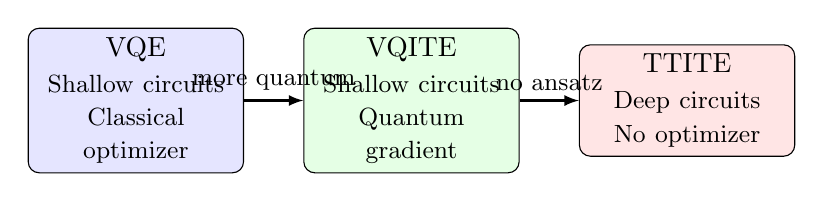
\begin{tikzpicture}[>=latex, node distance=3.5cm]
  \node[draw, rounded corners, fill=blue!10, text width=2.5cm, align=center]
    (vqe) {VQE\\[2pt]\small Shallow circuits\\Classical optimizer};
  \node[draw, rounded corners, fill=green!10, text width=2.5cm, align=center,
    right of=vqe] (vqite) {VQITE\\[2pt]\small Shallow circuits\\Quantum gradient};
  \node[draw, rounded corners, fill=red!10, text width=2.5cm, align=center,
    right of=vqite] (ttite) {TTITE\\[2pt]\small Deep circuits\\No optimizer};

  \draw[->, thick] (vqe) -- node[above, font=\small] {more quantum} (vqite);
  \draw[->, thick] (vqite) -- node[above, font=\small] {no ansatz} (ttite);
\end{tikzpicture}
\end{center}

VQE is the most practical for near-term noisy devices but offers the weakest
theoretical guarantees.  VQITE improves convergence reliability through
natural gradient dynamics but retains the ansatz limitation.  TTITE
eliminates the ansatz entirely and is exact in principle, but its
exponential postselection overhead limits practical applicability.

The upcoming apples-to-apples comparison will quantify these trade-offs on
a concrete problem, providing empirical evidence for which method offers the
best accuracy-per-quantum-resource on near-term hardware.


\end{document}
